\documentclass[tikz,border=6pt]{standalone}

\usepackage{tikz}
\usetikzlibrary{arrows.meta,positioning,fit,backgrounds}
\usepackage{xcolor}

\definecolor{networkblue}{RGB}{52,152,219}
\definecolor{envgreen}{RGB}{46,204,113}
\definecolor{algorange}{RGB}{230,126,34}
\definecolor{allocpurple}{RGB}{155,89,182}
\definecolor{deepnavy}{RGB}{27,42,73}
\definecolor{textgray}{RGB}{68,68,68}

\begin{document}
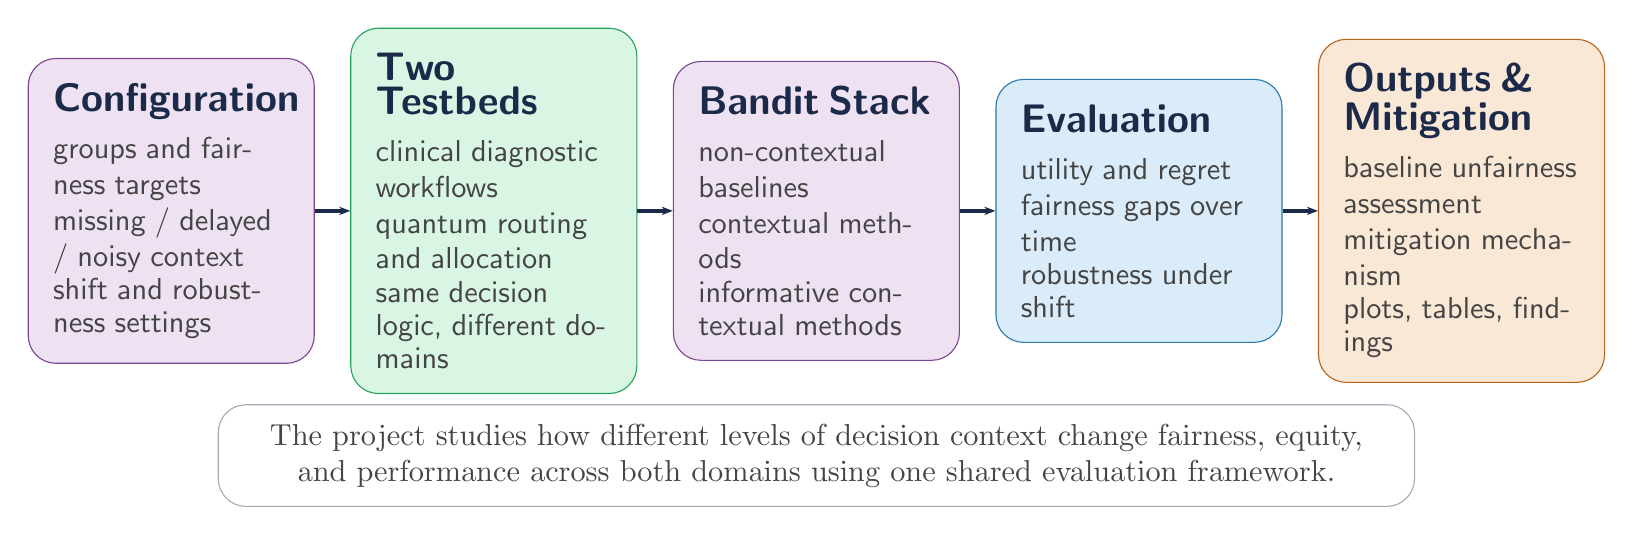
\begin{tikzpicture}[
  font=\sffamily,
  >={Stealth[length=4pt]},
  stage/.style={
    rectangle,
    rounded corners=10pt,
    draw=#1!80!black,
    fill=#1!18,
    text width=3.0cm,
    minimum height=2.65cm,
    align=left,
    inner sep=9pt
  },
  arrow/.style={->, line width=1.2pt, draw=deepnavy}
]

\node[stage=allocpurple] (config) {
  {\bfseries\fontsize{15}{17}\selectfont\color{deepnavy} Configuration}\\[4pt]
  {\fontsize{11}{13}\selectfont\color{textgray}
  groups and fairness targets\\
  missing / delayed / noisy context\\
  shift and robustness settings}
};

\node[stage=envgreen, right=0.45cm of config] (testbeds) {
  {\bfseries\fontsize{15}{17}\selectfont\color{deepnavy} Two Testbeds}\\[4pt]
  {\fontsize{11}{13}\selectfont\color{textgray}
  clinical diagnostic workflows\\
  quantum routing and allocation\\
  same decision logic, different domains}
};

\node[stage=allocpurple, right=0.45cm of testbeds] (bandits) {
  {\bfseries\fontsize{15}{17}\selectfont\color{deepnavy} Bandit Stack}\\[4pt]
  {\fontsize{11}{13}\selectfont\color{textgray}
  non-contextual baselines\\
  contextual methods\\
  informative contextual methods}
};

\node[stage=networkblue, right=0.45cm of bandits] (eval) {
  {\bfseries\fontsize{15}{17}\selectfont\color{deepnavy} Evaluation}\\[4pt]
  {\fontsize{11}{13}\selectfont\color{textgray}
  utility and regret\\
  fairness gaps over time\\
  robustness under shift}
};

\node[stage=algorange, right=0.45cm of eval] (outputs) {
  {\bfseries\fontsize{15}{17}\selectfont\color{deepnavy} Outputs \& Mitigation}\\[4pt]
  {\fontsize{11}{13}\selectfont\color{textgray}
  baseline unfairness assessment\\
  mitigation mechanism\\
  plots, tables, findings}
};

\draw[arrow] (config.east) -- (testbeds.west);
\draw[arrow] (testbeds.east) -- (bandits.west);
\draw[arrow] (bandits.east) -- (eval.west);
\draw[arrow] (eval.east) -- (outputs.west);

\node[
  draw=deepnavy!40,
  rounded corners=10pt,
  fill=white,
  inner sep=7pt,
  text width=14.7cm,
  align=center,
  below=0.55cm of bandits.south,
  font=\fontsize{11}{13}\selectfont,
  text=textgray
] (note) {
  The project studies how different levels of decision context change fairness, equity,
  and performance across both domains using one shared evaluation framework.
};

\end{tikzpicture}
\end{document}
